\chapter{複眼の光学的特性}
\label{CKnowledge}

本章では、昆虫や甲殻類に見られる複眼に関する知識や研究を紹介する。

\section{眼の種類}

自然界に存在する眼の形態は主に単眼、複眼、カメラ眼に別れており、特に人や哺乳類のカメラ眼と昆虫や甲殻類などの複眼には大きな違いがある。
カメラ眼は取り込む光量の調節機能や、ピント調節機能をそなえた、いわゆるカメラと同様の構造をもつ眼である\cite{newton-2012-6}。
脊椎動物の魚類、両生類、爬虫類、鳥類、哺乳類はあ基本的に同じ構造のカメラ眼をもち、無脊椎動物でもイカやタコの仲間が例外的にカメラ眼をもつ\cite{newton-2012-6}。


%% カメラ眼とは、ピントの調整を行える可動な1枚の大きなレンズまたは水晶体、取り込む光量を調整する機能、そして網膜のような面積が広い光受容組織を供えた、いわゆるカメラと基本的に同じ構造を持つ目である。これは大型の動物でも比較的小さな目で視力を持つのに適し、すべての脊椎動物が備えている\cite{}。角膜やレンズを持った事で像を結ぶ点に優れ、さらにレンズを動かす筋肉を発達させたため遠くを見る事でも有利である\cite{}。

\section{複眼の性質}

自然界に存在する眼の形態は主に単眼、複眼、カメラ眼に別れており、とくに複眼とカメラ眼は最も高度であるとされている\cite{newton-2012-6}。
カメラ眼は取り込む光量の調節機能や、ピント調節機能をそなえた、いわゆるカメラと同様の構造をもつ眼である\cite{newton-2012-6}。
脊椎動物の魚類、両生類、爬虫類、鳥類、哺乳類はあ基本的に同じ構造のカメラ眼をもち、無脊椎動物でもイカやタコの仲間が例外的にカメラ眼をもつ\cite{newton-2012-6}。

一方、複眼は個眼と呼ばれる単位の視覚器官から構成される\figref{FOmmatidia}。
ひとつの個眼にはレンズと光受容細胞(photoreceptor cell)および色素細胞(pigment cell)などが含まれる。
一般に、複眼を構成する個眼の数は複眼の大きさに比例し、ハエなどの少ないものでは数百個、トンボなどの多いものでは2万個以上であると言われている\cite{arikawa-zougan}。
一般に、昆虫や甲殻類などの外骨格をもつ生物が複眼をもつ。

\begin{figure}[hn]
  \centering
  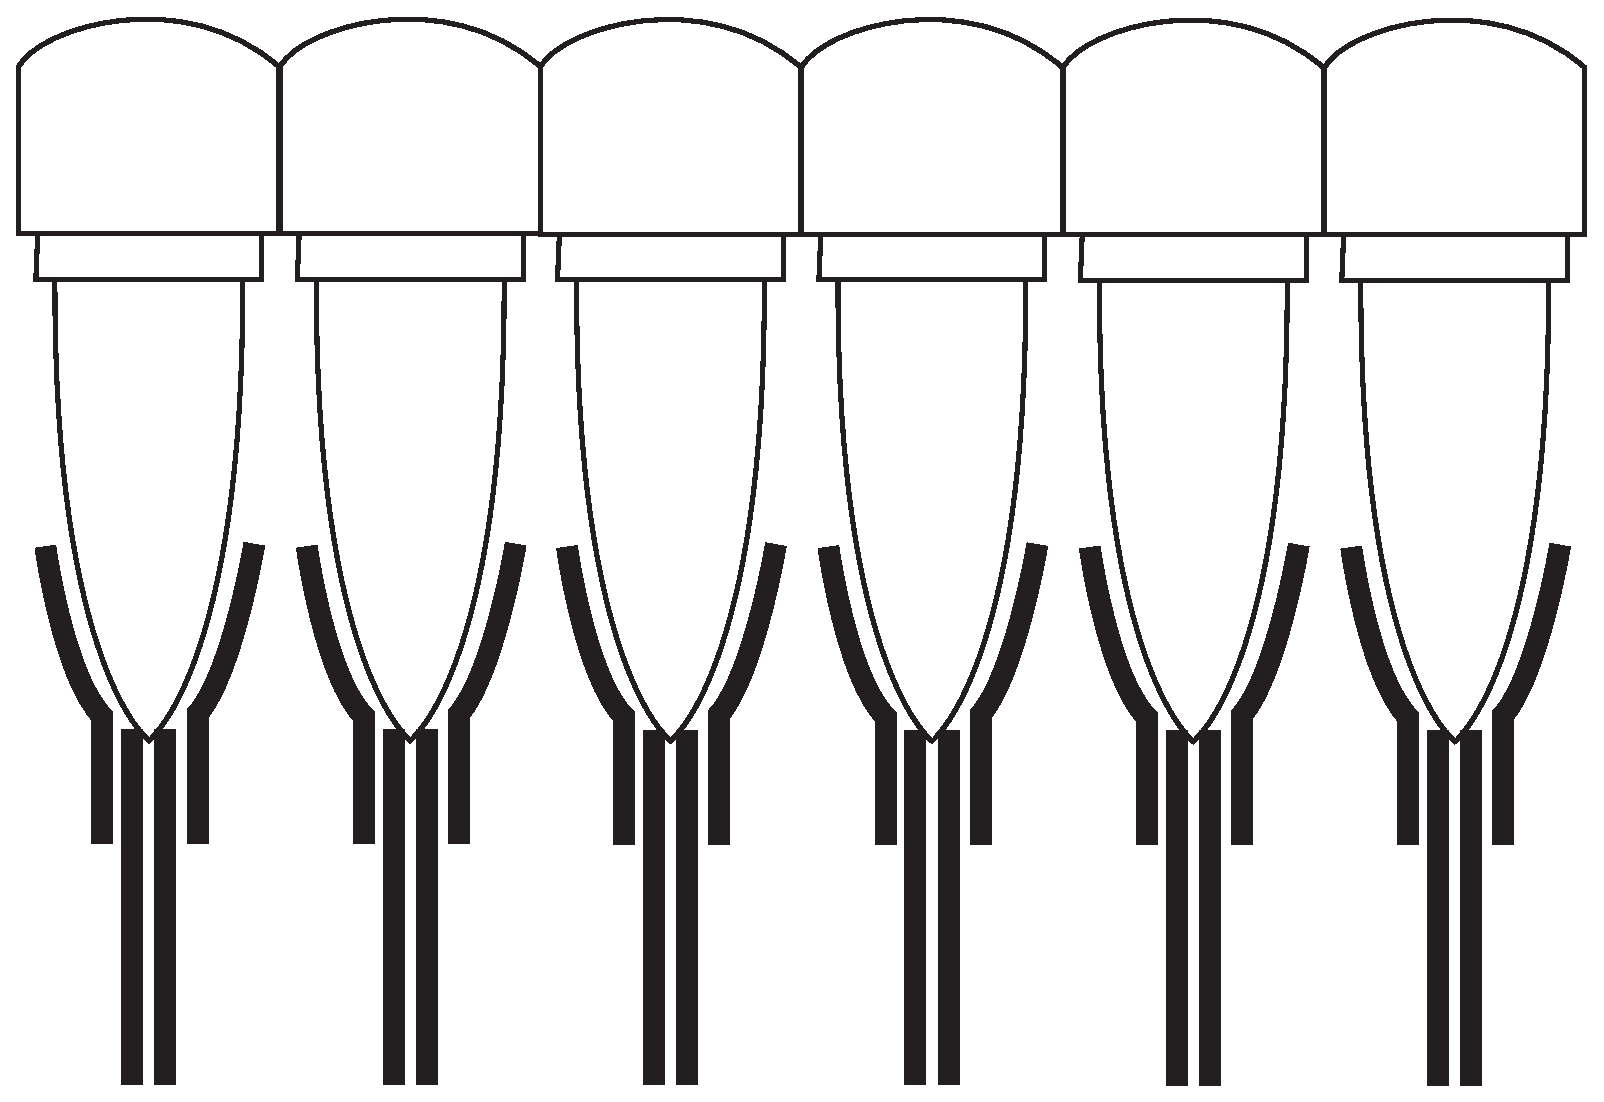
\includegraphics[width=4.0in]{./img/ommatidia.eps}
  \caption{個眼の模式図}
  \label{FOmmatidia}
\end{figure}

八木\cite{yagi1951studies}によると、昆虫に見られる複眼には複数のタイプがあり、真円錐眼(eucone eye)、偽円錐眼(pseudocone eye)、無円錐眼(acone eye)、外円錐眼(exocone eye)の4種類に大別される。
真円錐眼は堅いキチン質の円錐晶体をもち、独特な光学的性質を有している。
偽円錐眼は流動体もしくは半流動体で満たされたカプセルから構成され、比較的弱い屈折力しか持ち合わせていない。
無円錐眼は円錐晶体を有しておらず、外円錐眼では円錐晶体が角膜面のくぼみによって置き換えられている。
真円錐眼はさらに連立像眼\figref{FRenritsu}と重複像眼\figref{FTyoufuku}に分けられる。

\subsection{連立像眼}

チョウなどの眼は連立像眼(apposition eye)と呼ばれ、昼行性の種に多く見られる。
感覚神経のユニットは円錐晶体の頂点から離れ、ひとつずつ独立して光を受容するような構造になっている\cite{arikawa-zougan}。
すなわち、ひとつひとつの個眼は光学的に独立しており、レンズ直下の感桿に導かれた光は外に漏れることなく感桿基部まで到達する。
Nilsson\cite{nilsson1989optics}によると連立像眼はさらに少なくとも4タイプに分類され、単純連立型、無限焦点型(afocal type)、分散感桿型(open rhabdom)・神経重複型(nural superposition)、透明連立型などがある。
単純連立像眼と無限焦点連立像眼の基本構造はほぼ同じであるが、無限焦点連立像眼では単純連立像眼とは異なり感桿へ平行光が入射する。
蟻川\cite{arikawa-zougan}によると、単純連立型はハチ類やカニ類に多く見られ、無限焦点型はチョウ類で発見されたタイプであると言われている。
また、分散感桿型・神経重複型はハエ類などの一部の昆虫に見られ、透明連立型は浮遊性の甲殻類にのみ発見されている特殊なタイプであると言われている。

\begin{figure}[hn]
  \centering
  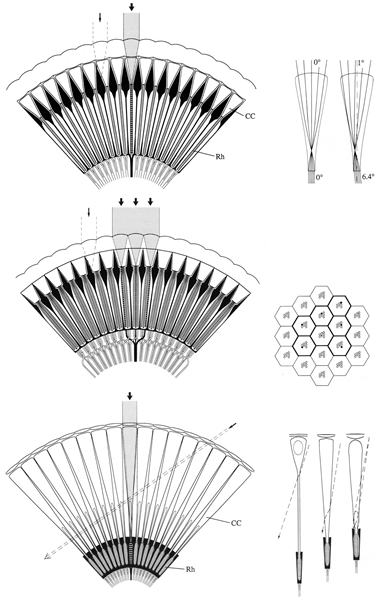
\includegraphics[width=3.0in]{./img/renrituzougan.jpg}
  \caption{連立像眼のしくみ(\cite{arikawa-zougan}より転載)}
  \label{FRenritsu}
\end{figure}

%% \begin{figure}[hn]
%%   \centering
%%   
\includegraphics[width=3.0in]{./img/TEMP}
%%   \caption{連立像眼の例}
%%   \label{FExpparts}
%% \end{figure}

\subsection{重複像眼}

連立像眼が昼行性の種に多く見られるのに対して、重複像眼はガなどの夜行性の種に多く見られる。
重複像眼の特徴としては、色素細胞の色素粒子が光の明暗によって上下に移動する点が挙げられる。
重複像眼の色素細胞は暗いところでは円錐晶体を取り囲むように上部へ移動する。
夜行性の昆虫などの眼が真っ黒に見えることと関連があると考えられる。

\begin{figure}[hn]
  \centering
  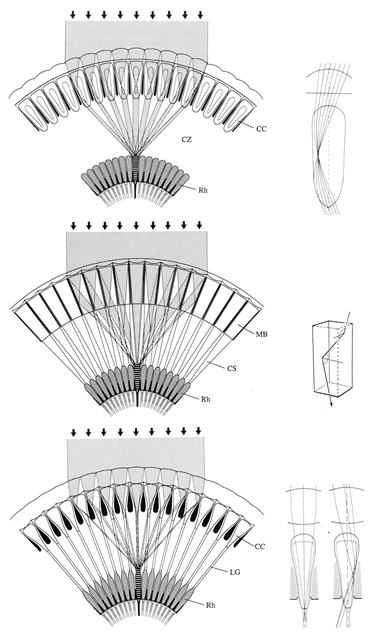
\includegraphics[width=3.0in]{./img/tyoufukuzougan.jpg}
  \caption{重複像眼のしくみ(\cite{arikawa-zougan}より転載)}
  \label{FTyoufuku}
\end{figure}

%% \begin{figure}[hn]
%%   \centering
%%   
\includegraphics[width=3.0in]{./img/TEMP}
%%   \caption{重複像眼の例}
%%   \label{F}
%% \end{figure}

\section{個眼のしくみ}

一般に、複眼が多数の小さな個眼の集合体であり、半球状のドームを形成していることはよく知られている。
個眼の表面は凸レンズ構造をしており、それぞれの形状は六角形もしくは正方形である\figref{FFukuganKakudai}。
個眼のひとつひとつは主にレンズ、色素細胞、円錐晶体そして感桿などから構成されており、複眼の偽瞳孔に関係が深く、外部的な見た目に影響する部位はレンズおよび色素細胞である。
\begin{figure}[htbp]
  \centering
  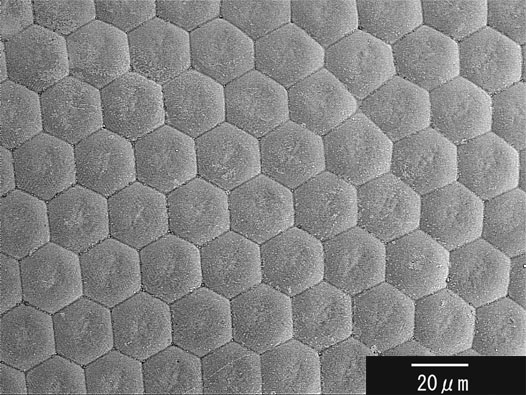
\includegraphics[width=3.0in]{./img/fukugan_kakudai.jpg}
  \caption{複眼表面の拡大画像(\cite{tinycafe}より転載)}
  \label{FFukuganKakudai}
\end{figure}

\section{偽瞳孔}
\label{SPseudopupil}

\secref{SObjective}で述べた偽瞳孔についてより詳細な説明を行う。 
偽瞳孔は複眼表面に見られる暗い斑点状の模様であり\figref{FWhatIsPseudopupil}、チョウやトンボ、セミなどさまざまな昆虫で顕著に現れる。
また、昆虫だけではなくエビやカニなどの複眼を持つ甲殻類にも見られる。

%% \begin{figure}[hn]
%%   \centering
%%   
\includegraphics[width=3.0in]{./img/TEMP}
%%   \caption{昆虫に見られる偽瞳孔}
%%   \label{F}
%% \end{figure}

%偽瞳孔の性質や観察による模様の違いなどを扱った研究は散見されるものの、幾何学的な構造と現れる模様とを関連付けて論じた研究は少ない。
%% Leydig\cite{}は{\it Limulus}(アメリカカブトガニ属)の複眼において瞳孔のような暗い斑点、すなわち偽瞳孔を観測し、脊椎動物の瞳孔とは違って外部から観察する方向によって斑点の位置が変化することに言及している。

基本的には、偽瞳孔は中心に位置する暗点とそれを取り囲む6つの暗点から構成されている。
周囲にある6つの暗点は中心の暗点を取り囲む六角形の頂点の位置に見られる。
八木\cite{yagi1951studies}は、これらの点のうち中心に位置する暗点をcentral pupil、周囲の位置にある6つの暗点をside pupilと呼称している。
また、side pupilの外側を取り囲むように配置される暗点も存在し、ひとつめのside pupilを中心として先述と同様に六角形状に位置する。
これらの暗点のうち、central pupilとside pupilをのぞいたものはsecond side pupilと呼称されている。
本研究でもこれらの呼称をそのまま用いることにする。

\subsection{Central Pupil}
\label{SSCentralPupil}

八木は色素細胞の位置によってcentral pupilの形状の変化が見られることについて記述している。
色素細胞が円錐晶体の下端にある場合\figref{FYagi4-3types}、central pupilは比較的丸い形状の単純な暗点として現れる。
この場合、色素細胞が少し円錐晶体の上部へ移動した場合と比較すると大きさはやや小さい。
色素細胞が少しだけ上部へ移動した場合には、偽瞳孔は少し大きくなり暗さを増す。
また、色素細胞がさらに移動し、レンズの近くまで上がってきた場合には、偽瞳孔の形状が六角形に近づいていくという。

\begin{figure}[htn]
  \centering
  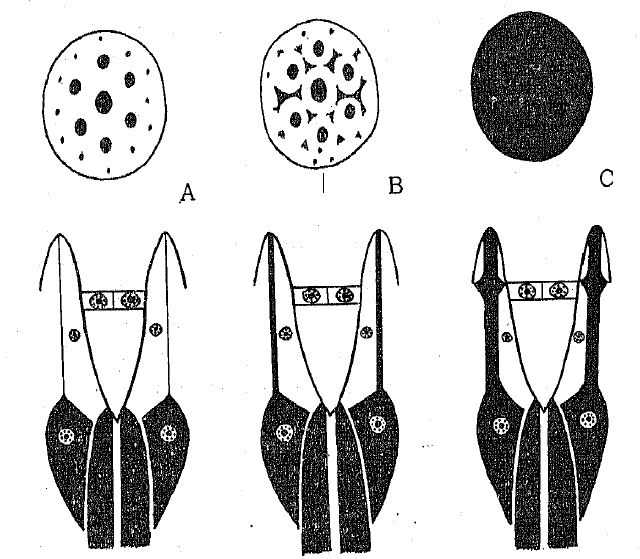
\includegraphics[width=3.5in]{./img/yagi4-3types.png}
  \caption{色素細胞の上下移動と偽瞳孔(\cite{yagi1958studies}より転載)}
  \label{FYagi4-3types}
\end{figure}

また、八木は以下のようにも述べている。
全ての偽瞳孔に当てはまるわけではないが、central pupilの中央には茶色もしくは赤みがかった明るい点を示すものがある。
これは、感桿を通して基底膜から反射した光によるものである。
しかしながら、この明点は一部の種をのぞいた他の種ではほとんど見られない。
なぜなら、色素細胞が基底部で円錐晶体を囲っており基底膜への光の進入を抑えているからである。
重複像眼では基底膜および気管のタペータム(tapetum:輝板)からの反射が合わさって赤もしくは琥珀色の明るい輝きになる。

\subsection{Side Pupil}
\label{SSSidePupil}

Side pupilはcentral pupilから同距離に位置し、色素細胞からの間接反射によって起こる。
Central pupilは光が入射したレンズが属している個眼の色素細胞の色を反射しているが、side pupilは光が入射したレンズが属している個眼に隣接する個眼の色素細胞からの反射によって生じる\cite{yagi1951studies}。

光が\figref{FSidepupilexplanation}のAのような道筋を通る場合、この個眼の表面はcentral pupilの一部として観測される。
一方、光が\figref{FSidepupilexplanation}のCのような道筋を通る場合、この個眼の表面はside pupilの一部として観測される。
円錐晶体には色素細胞に覆われている部分と覆われていない部分がある。
\figref{FSidepupilexplanation}のBおよびDの道筋を通る視線は、色素細胞に覆われていない円錐晶体の一部に到達している。
通常、これらの位置にぶつかった光は円錐晶体の奥にある体液の色を反射し薄い色として観測される\cite{yagi1951studies}。

角度を変えながらひとつの個眼のレンズを観測すると、ある特定の角度の範囲内で円錐晶体の壁面に沿った色素細胞の色を反射することは明らかである。
逆に、円錐晶体において色素細胞のない壁面の色を反射する角度の範囲も存在すると言える。
すなわち、複眼表面においてcentral pupilとside pupilの間には色素のない領域が存在することは想像に難くない。
また、second side pupilの生じる原理も同様である。

\begin{figure}[htn]
  \centering
  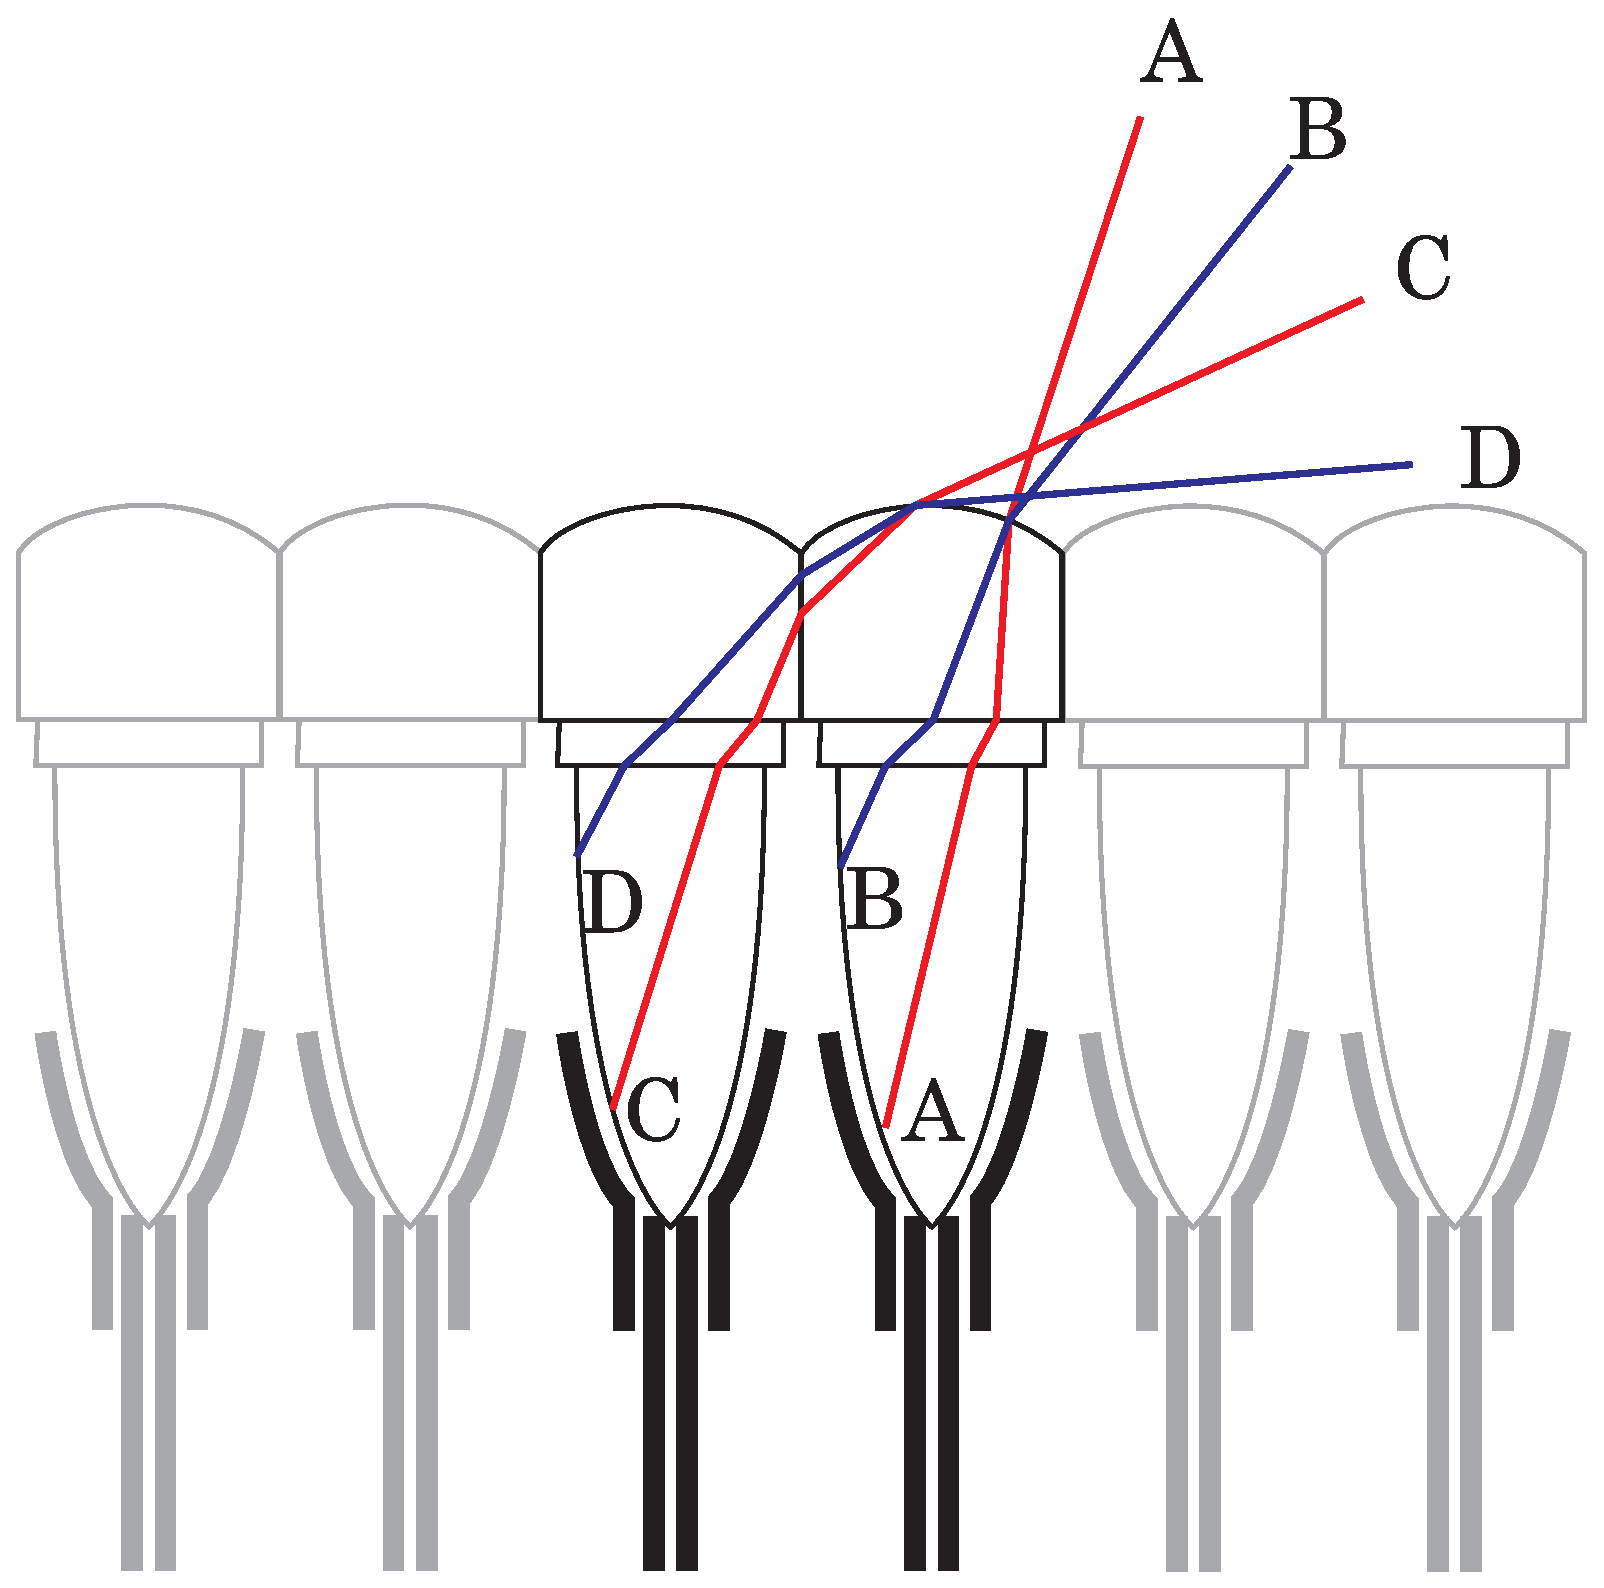
\includegraphics[width=3.5in]{./img/sidepupil_exp}
  \caption{Side pupilの原理}
  \label{FSidepupilexplanation}
\end{figure}

偽瞳孔の暗点はcentral pupil, side pupil, second side pupilの順に色が薄く見えるものも存在する。
その理由としては、side pupilおよびsecond side pupilは隣接する個眼を通過して色素細胞の色を反射するため、通過する個眼のレンズや体液が厚くなり、光が減衰するからであると推測される。

